% !Mode:: "TeX:UTF-8"

\chapter{两轮平衡车结构设计与控制系统研究}

对载人两轮平衡车进行需求分析，确定两轮平衡车进行总体设计方案。确定具体性能设计指标，对两轮平衡车的结构进行结构设计并对关键零部件进行强度校核或有限元分析；根据两轮平衡车的控制需求进行控制系统方案设计，进行元器件选型搭建硬件环境，并设计控制系统的软件框架。

\section{总体设计}

两轮平衡车作为一种新型的个人短途代步工具，其应用场景已从最初的休闲娱乐扩展到城市微出行、景区观光、园区通勤等多个领域。本课题针对公园环境中使用的载人两轮平衡车进行设计研究，具体需求如下：

（1）安全稳定性：要求车辆在行驶和静止状态下均具备良好的稳定性能，尤其在坡道、弯道及复杂地形中能够有效防止倾倒或失控现象的发生；

（2）乘坐舒适性：座椅设计应符合人体工程学原理，提供良好的支撑与减震效果，提升乘坐体验；

（3）操作灵活性：转向和加减速响应需灵敏可靠，适应公园内狭窄、弯曲、起伏等多样化路径，满足低速频繁启停的使用特点；

（4）使用便捷性：支持手机APP远程叫车与还车功能，实现无人自主行驶状态下的“召之即来，挥之即去”，提升用户使用便利性；

（5）行驶安全性：在自动行驶模式下，应具备环境感知、路径规划及动态避障能力，确保在复杂多变的公园环境中实现安全、顺畅的通行。

\begin{figure}[!htbp]
  \centering
  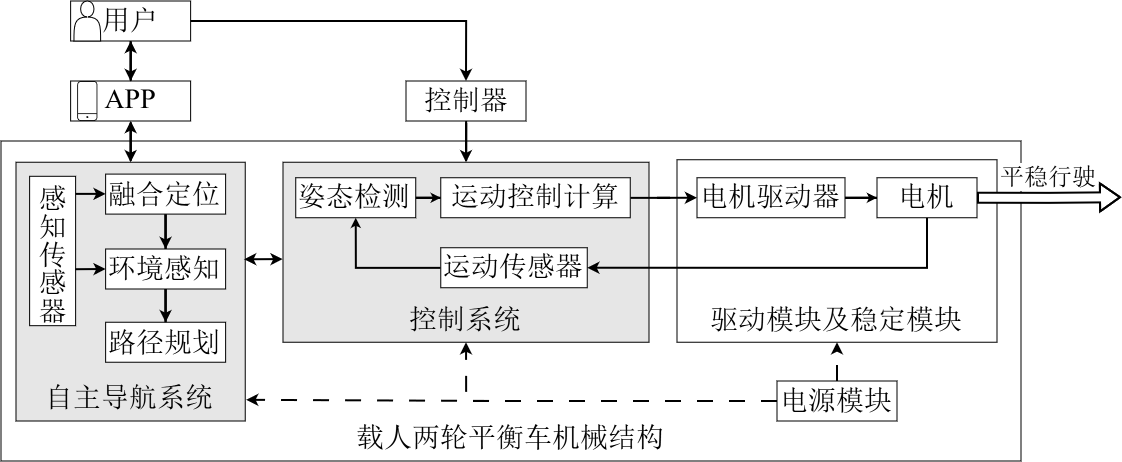
\includegraphics[width=0.85\textwidth]{figures/chapter02/载人两轮平衡车总体设计方案.png}
  \caption{载人两轮平衡车总体设计方案}
  \label{载人两轮平衡车总体设计方案}
\end{figure}

基于上述需求分析，本课题提出了一种载人两轮平衡车的设计方案，如图\ref{载人两轮平衡车总体设计方案}所示。从整体架构上看，载人两轮平衡车系统主要由三大核心部分组成：机械结构、控制系统与自主导航系统。三者密切协作、相互配合，共同实现平衡车的稳定运行与自主行驶。各部分的具体功能与组成如下：

（1）机械结构：载人两轮平衡车机械结构为车体提供结构支撑，并为整车的行驶与平衡控制提供动力。其主要包括车体框架、驱动模块以及稳定模块；

（2）控制系统：载人两轮平衡车的控制系统主要负责整车的运动与姿态控制。系统能够接收运动指令，实时采集运动传感器数据，进行控制计算，调节电机输出，实现车辆的平衡控制与行驶操作；

（3）自主导航系统：载人两轮平衡车的自主导航系统主要功能是通过传感器实现定位与环境感知，进而进行路径规划与避障控制，保障车辆在复杂环境中的自主导航与安全行驶。

\begin{figure}[!htbp]
  \centering
  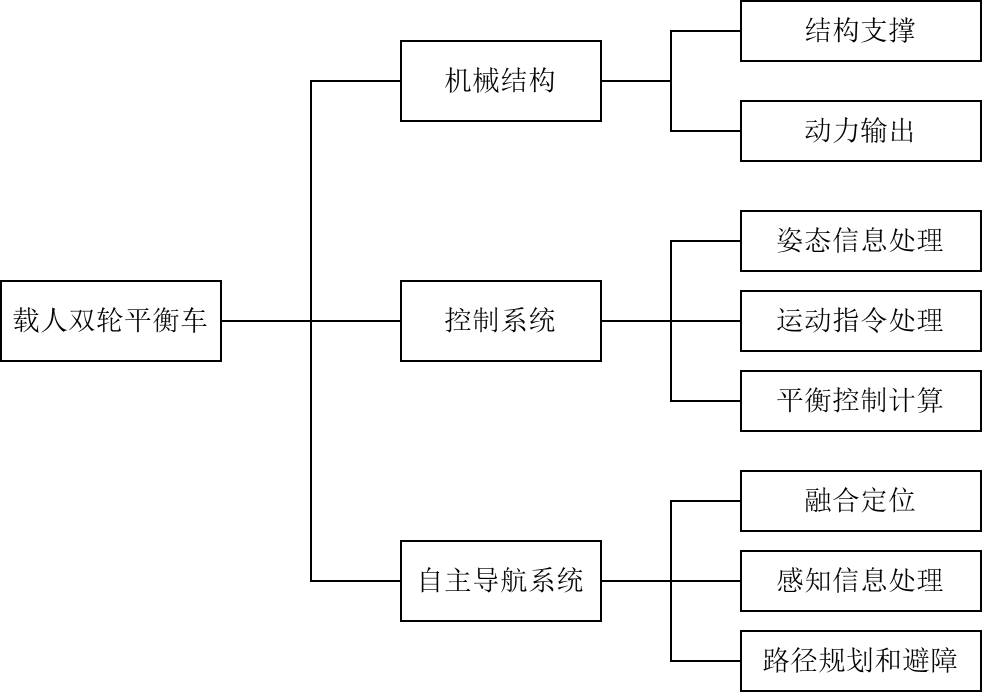
\includegraphics[width=0.85\textwidth]{figures/chapter02/载人两轮平衡车系统功能组成图.png}
  \caption{载人两轮平衡车系统功能组成图}
  \label{载人两轮平衡车系统功能组成图}
\end{figure}

\section{机械结构设计}

根据两轮平衡车的需求进行机械结构设计。首先，根据确定设计指标，进行两轮平衡车的结构方案设计；然后，根据功能将结构划分为不同的部分，进行各部分的详细设计及校核；最后进行对关键结构进行有限元分析。

\subsection{机械结构设计方案}

载人两轮平衡车的设计指标如表\ref{两轮平衡车设计指标}所示。因使用场景在公园、社区等生活场所，外形尺寸参照《GB/T 12996-2023 电动轮椅车》确定为不超过总长不超过900mm且总宽不超过750mm；参考国家国民体质监测中心发布的《第五次国民体质监测公报》中成年人的体重确定额定载荷为75kg。

\begin{table}[!htbp]
  \centering
  \caption{两轮平衡车设计指标}
  \label{两轮平衡车设计指标}
  \vspace{0.5em}\wuhao
  \begin{tabularx}{\textwidth}{>{\centering\arraybackslash}X>{\centering\arraybackslash}X>{\centering\arraybackslash}X}
    \toprule
    指标分类 & 指标项目 & 具体要求 \\
    \midrule
    尺寸 & 总长 & ≤900mm \\
     & 总宽 & ≤750mm \\
     & 整车质量 & 70kg \\
    运动性能 & 额定载荷 & 75kg \\
     & 最大运动速度 & 15km/h \\
     & 最大加速度 & 2m/s2 \\
     & 爬坡性能 & 15° \\
    \bottomrule
  \end{tabularx}
\end{table}

本课题设计的载人两轮平衡车需兼顾安全性与舒适性。传统两轮平衡车通常基于倒立摆原理实现平衡控制，但该结构本质上属于不稳定系统，易在速度变化或外部扰动时产生倾斜与位移。以Segway为代表的传统平衡车利用这一特性，通过人体倾斜改变重心以控制运动。而本课题中的平衡车面向乘坐式应用，用户通过控制器发送运动指令进行操控，不再依赖身体姿态调节，这对车辆的稳定性和响应性提出更高要求。为了提升系统在复杂工况下的稳定性与乘坐舒适性，本设计在传统倒立摆控制基础上引入力矩控制陀螺（Control Moment Gyroscope，CMG），通过提供快速、精确的姿态调节力矩，有效应对由加减速或外部扰动引起的倾斜问题，从而增强整体的动态平衡性能。因此，本课题采用倒立摆控制与力矩控制陀螺联合控制方案，以实现更高水平的稳定性与操控性。

根据上述控制方案，载人两轮平衡车的机械结构可以分为三部分：车体框架、稳定模块和驱动模块。

（1）车体框架作为整车的承载基础，主要用于安装各类硬件组件，并为乘员提供稳固的乘坐空间；

（2）稳定模块用于增强车辆在动态行驶过程中的姿态稳定性，通过集成力矩控制陀螺结构，在车辆受到加减速或外部扰动时提供额外的控制力矩，以提升平衡性能和乘坐舒适性；

（3）驱动模块包括电机和轮组，是整车的动力输出单元，负责将控制系统的指令转化为实际运动，实现车辆的加速、减速及转向等基本行驶功能，同时为平衡控制提供必要的动态响应能力。

\subsection{车体框架设计}

车体框架的主要功能包括承载驱动模块、稳定模块以及其他辅助零部件。本课题设计的双轮平衡车采用了模块化设计、具有装拆方便、集成度高的特点。车体框架如图\ref{两轮平衡车车体框架设计示意图}所示，整体结构主要由车体前后左右四个侧板和两个连接架组成。

\begin{figure}[!htbp]
  \centering
  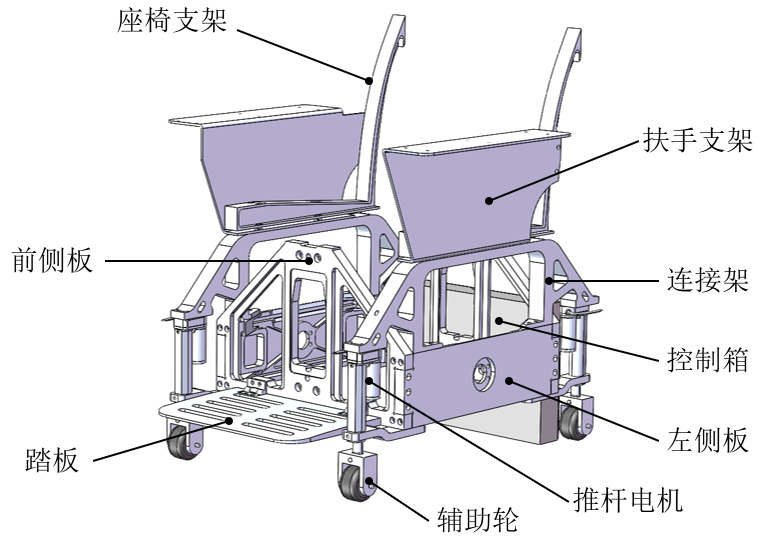
\includegraphics[width=0.85\textwidth]{figures/chapter02/两轮平衡车车体框架设计示意图.png}
  \caption{两轮平衡车车体框架设计示意图}
  \label{两轮平衡车车体框架设计示意图}
\end{figure}

车体前侧板用于安装踏板，后侧板安装控制箱以集成控制系统；左右两侧板则作为驱动模块的安装基座固定电机和车轮。四块侧板共同围成一个稳定模块的封闭安装腔体，为后续稳定模块的布置提供充足空间，并有助于整车质量分布的均衡及重心的合理控制，从而提升车体运行的稳定性。

两个连接架安装在左右两侧板上，用于安装其他辅助零部件，包括扶手支架和座椅支架，此外在支撑架的前后两段各安装有集成推杆电机的辅助支撑轮用于车辆在启停和维修时的辅助支撑。

连接架分别安装于左右侧板上，作为安装其他辅助零部件的基座。两连接架上固定有扶手支架与座椅支架，确保乘坐结构的稳固与承重能力。此外，在每个连接架的前后端下均安装有集成推杆电机的辅助支撑轮组件，用于在车辆启动、停止或维修过程中提供临时支撑，提升整车的操作便利性与使用安全性。

在设计乘坐空间时，参考《GB/T 10000-2023中国成年人人体尺寸》和《GB/T 3326—2016椅、凳类主要尺寸》，确定座椅有效宽度为520 mm、坐深430 mm、坐高400 mm，踏板长度不少于250 mm，以满足乘坐舒适性的基本要求。

车体框架采用铝合金6061材料，车体框架设计使用的是三维设计软件Solidworks，这款软件具备直观的3D开发环境,可以对复杂的产品进行高效的建模,也支持将建好的移动机器人模型导入到Ansys中，方便后续对结构进行物理仿真。

\subsection{稳定模块设计}

稳定模块是载人两轮平衡车安全性和舒适性的重要保证，其集成力矩控制陀螺以平衡倒立摆所产生的倾角摆动。首先说明力矩控制螺的原理和双陀螺布置结构；然后对主要结构进行设计。

（1）力矩控制陀螺原理及布置结构

力矩控制陀螺是一种通过改变飞轮方向以产生控制力矩的装置，广泛应用于航天器姿态控制和高动态平衡系统中。力矩控制陀螺的结构主要包括高速旋转的飞轮、陀螺壳体以及外部安装框架。如图\ref{陀螺力矩方向示意图}所示飞轮绕自身主轴（图中 $y$ 轴）以角速度 $\omega_y$ 高速旋转，形成稳定的角动量矢量。当通过控制电机驱动其绕垂直于飞轮轴线的 $z$ 轴以角速度 $\omega_z$ 进动时，根据角动量守恒定律，系统将产生垂直于两轴的进动力矩 $\tau$，其方向沿 $x$ 轴指向。

\begin{figure}[!htbp]
  \centering
  \begin{minipage}[t]{0.48\textwidth}
    \centering
    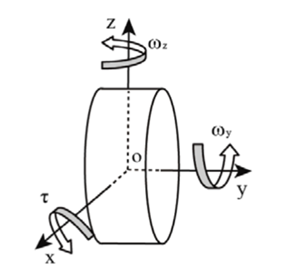
\includegraphics[width=\textwidth]{figures/chapter02/陀螺力矩方向示意图.png}
    \caption{陀螺力矩方向示意图}
    \label{陀螺力矩方向示意图}
  \end{minipage}
  \hfill
  \begin{minipage}[t]{0.48\textwidth}
    \centering
    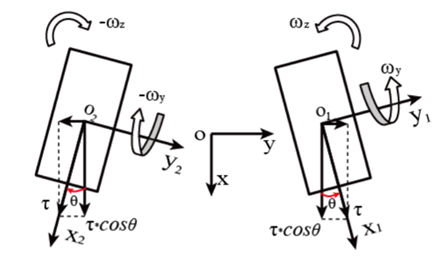
\includegraphics[width=\textwidth]{figures/chapter02/双CMG结构示意图.png}
    \caption{双CMG结构示意图}
    \label{双CMG结构示意图}
  \end{minipage}
\end{figure}

力矩控制陀螺产生的进动力矩来源于角动量的变化率。若设飞轮角动量L为：
\begin{equation}
L = I_y \omega_y \mathbf{e}_y
\end{equation}

\noindent \begin{tabularx}{\textwidth}{@{}l@{\quad}r@{———}X@{}}
式中& $L$ & 飞轮角动量（kg·m$^2$/s）；\\
& $I_y$ & 飞轮对自转轴的转动惯量（kg·m$^2$）；\\
& $\omega_y$ & 飞轮的自转角速度（rad/s）；\\
& $\mathbf{e}_y$ & $Y$轴方向的单位向量。\\
\end{tabularx}\vspace{3.15bp}

则当飞轮绕 $z$ 轴旋转时，其角动量方向随之发生变化，进而产生进动力矩，该力矩的大小与飞轮转速 $\omega_z$、进动角速度 $\omega_y$ 成正比，方向由右手定则确定：
\begin{equation}
\tau = \frac{\mathrm{d}L}{\mathrm{d}t} = I_y \omega_y \omega_z \mathbf{e}_x
\end{equation}

\noindent \begin{tabularx}{\textwidth}{@{}l@{\quad}r@{———}X@{}}
式中& $\tau$ & 飞轮产生的进动力矩（N·m）；\\
& $\omega_z$ & 飞轮的进动角速度（rad/s）；\\
& $\mathbf{e}_x$ & $X$轴方向的单位向量。\\
\end{tabularx}\vspace{3.15bp}

然而单个CMG在产生进动力矩的同时，也会由于结构偏置产生附加力矩分量，影响整体系统的稳定性。如图\ref{双CMG结构示意图}所示在存在倾角 $\theta$ 的情况下，CMG所产生的进动力矩 $\tau$ 可分解为沿 $x$ 轴方向的分力矩 $\tau \cos\theta$，从而引入非期望的扭矩分布。为此采用对称双CMG布置结构是一种有效的抑制手段。两组CMG沿相同轴线对称放置，飞轮自转方向相反，进动方向也相反，最后产生的合力矩的方向沿绝对坐标系 $X$，两个陀螺在绝对坐标 $Y$ 轴方向产生的分力矩相互抵消。采用双陀螺布置的力矩控制陀螺装置产生的控制力矩为：
\begin{equation}
\tau = 2 I_y \omega_y \omega_z \mathbf{e}_x \cos\theta
\label{eq:ch2-cmg-double}
\end{equation}

\noindent \begin{tabularx}{\textwidth}{@{}l@{\quad}r@{———}X@{}}
式中& $\theta$ & 飞轮转动角（$^\circ$）。\\
\end{tabularx}\vspace{3.15bp}

采用双陀螺布置结构显著降低系统由飞轮自转引入的耦合扰动，提升控制稳定性与响应灵敏度，所以稳定模块的力矩控制陀螺采用双陀螺布置结构。根据式~\eqref{eq:ch2-cmg-double}，力矩控制陀螺产生的控制力矩与转子的转动惯量、自转角速度和进动角速度成正比。由于飞轮自转速度较高不易调整，一般由高速电机保持自转速度恒定，通过调节进动角速度来控制所需的平衡力矩。

（2）稳定模块结构设计

稳定模块结构如图\ref{稳定模块结构}，主要由力矩控制陀螺装置、调节机构及电池包构成。

\begin{figure}[!htbp]
  \centering
  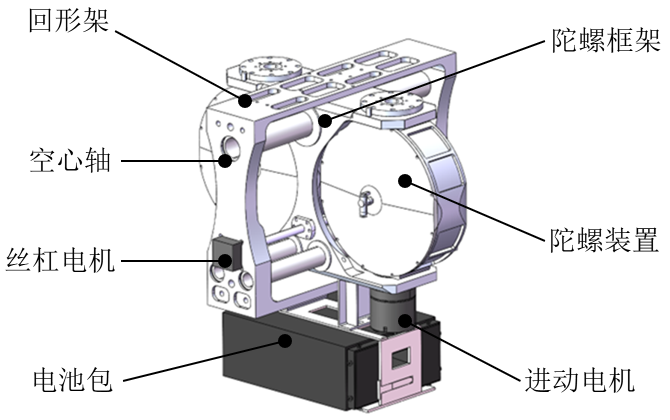
\includegraphics[width=0.85\textwidth]{figures/chapter02/稳定模块结构.png}
  \caption{稳定模块结构}
  \label{稳定模块结构}
\end{figure}

力矩控制陀螺装置由两个对称布置的陀螺装置、进动电机以及陀螺框架组成。每个陀螺装置包含飞轮、高速电机和陀螺外壳，并通过连接轴与轴承固定于陀螺框架上。进动电机用于驱动陀螺装置的进动，实现对其进动角速度的精确控制。陀螺外壳及安装支架选用铝合金6061制造，该材料具有良好的力学性能与加工性能；飞轮部分则采用密度较大的45号钢，以显著提高陀螺转子的转动惯量，从而在进动过程中产生更大的进动力矩，增强姿态控制能力。

调节机构主要用于调节力矩控制陀螺的安装位置，其结构集成了回形架、空心轴以及丝杆电机。回形架采用铝合金6061材质材料，不仅为各子组件提供了安装平台，同时通过集成空心轴和丝杆电机构成高效的调节单元。此外为实现结构的紧凑布局，电池包采用下挂式安装方式，固定于陀螺框架的下方。

（3）进动电机的选型

稳定模块产生的控制力矩必须大于两轮平衡车倾斜时的重力矩。当平衡车载人状态下前后方向倾斜的角度为$\beta$时，产生的重力矩$T_G$为：
\begin{equation}
T_G = m_c g h_c \sin\beta + m_p g h_p \sin\beta
\end{equation}

\noindent \begin{tabularx}{\textwidth}{@{}l@{\quad}r@{———}X@{}}
式中& $m_c$ & 平衡车自重；\\
& $h_c$ & 平衡车重心高度；\\
& $m_p$ & 人体质量；\\
& $h_p$ & 人体乘坐时重心高度。\\
\end{tabularx}\vspace{3.15bp}

根据总体结构设计，估算$m_c=70\,\mathrm{kg}$，$h_c=0.42\,\mathrm{m}$，取$m_p=75\,\mathrm{kg}$，$h_p=0.85\,\mathrm{m}$，当$\beta=20^\circ$时代入计算得$T_G=312.64\,\mathrm{N\cdot m}$。所以稳定模块产生的控制力矩应不小于$312.64\,\mathrm{N\cdot m}$。

陀螺装置为根据车内空间设计的定制产品，其飞轮绕自转轴的转动惯量为$I_y=0.09\,\mathrm{kg/m^2}$，内部高速电机额定转速$\omega_y=471.24\,\mathrm{rad/s}$（4500rpm），CMG倾角$\theta=10^\circ$。由式~\eqref{eq:ch2-cmg-double}计算得进动角速度应不小于$3.75\,\mathrm{rad/s}$（35.81rpm）。

设进动角速度为$\omega_z=3.77\,\mathrm{rad/s}$（36rpm），为达到100Hz的控制周期，故需要在$0.01\,\mathrm{s}$的时间内加速到目标转速，其加速功率计算公式：
\begin{equation}
P_{\alpha} = \frac{\omega_z^2 J_z}{2 t_{\alpha}}
\label{eq:ch2-power-acc}
\end{equation}

\noindent \begin{tabularx}{\textwidth}{@{}l@{\quad}r@{———}X@{}}
式中& $P_{\alpha}$ & 加速功率（W）；\\
& $\omega_z$ & 进动角速度（rad/s）；\\
& $J_z$ & 陀螺绕进动轴的转动惯量（kg/m$^2$）；\\
& $t_{\alpha}$ & 加速时间（s）。\\
\end{tabularx}\vspace{3.15bp}

\noindent 考虑安全系数S=0.3，实际选择电机功率的额定功率应不小于P：
\begin{equation}
P = P_{\alpha}(1 + S)
\label{eq:ch2-power-rated}
\end{equation}

由式~\eqref{eq:ch2-power-acc}和式~\eqref{eq:ch2-power-rated}计算得进动电机的额定功率应大于34.82W。

电机所需的转矩$T$为：
\begin{equation}
T = \frac{J_z \omega_z}{t_{\alpha}}
\end{equation}

计算得进动电机所需的转矩为$18.47\,\mathrm{N\cdot m}$。

最终选择了RobStride03一体化关节电机，该电机集成了电机本体、减速器和驱动器，结构紧凑，适合车内安装。其详细参数如表\ref{进动电机技术参数}所示。

\begin{table}[!htbp]
  \centering
  \caption{进动电机技术参数}
  \label{进动电机技术参数}
  \vspace{0.5em}\wuhao
  \begin{tabularx}{\textwidth}{>{\centering\arraybackslash}X>{\centering\arraybackslash}X>{\centering\arraybackslash}X>{\centering\arraybackslash}X>{\centering\arraybackslash}X>{\centering\arraybackslash}X}
    \toprule
    型号 & 额定电压 & 额定转速 & 额定扭矩 & 峰值扭矩 & 额定功率 \\
    \midrule
    RobStride03 & 48V & 180RPM & 20Nm & 60Nm & 380w \\
    \bottomrule
  \end{tabularx}
\end{table}

\subsection{驱动模块设计}

驱动模块包括电机和车轮构成两轮差速驱动结构。首先通过整体尺寸及行驶需求估算并选择车轮大小；然后各工况下电机所需的扭矩、转速以及功率，并以此对电机进行选型，完成驱动模块的设计。

为提升车辆在园区砖缝、人行道起伏、减速带等半结构化环境下的通过性，参考《GB/T18029.10-2008轮椅第10部分：越障能力的测定》中关于可越过150 mm宽沟槽与80 mm高障碍物的推荐值，设定最小离地间隙不小于80 mm。该间隙由轮胎半径与底盘结构设计共同决定。为满足通过性与平衡稳定性要求，结合车身整体尺寸以及结构，选用直径26寸（660mm）的轮胎。

根据结构方案设计所述，本课题设计的两轮平衡车采用倒立摆与力矩控制陀螺联合控制的平衡方案。倒立摆需要通过电机驱动车轮实现，实现轮式倒立摆常用的电机有轮边电机或轮毂电机。轮边电机轮边电机具有成本低、维护方便、簧下质量小等优势，而轮毂电机则凭借更高的响应速度以及更紧凑的结构设计且不占用车内空间，选用轮毂电机能够更好地满足结构设计需求。

为保证车辆在各工况下具备良好的驱动能力，需要根据设计指标计算符合各种工况下电机所需的扭矩、转速以及功率。平衡车在行驶中受到的阻力主要有滚动摩擦阻力$F_r$、空气阻力$F_a$、坡道阻力$F_c$以及加速阻力$F_{ac}$，根据工况进行计算。

1）最大爬坡角度时的阻力

在爬坡时，平衡车需要克服滚动摩擦阻力和坡道阻力，因速度较低忽略空气阻力。最大爬坡角度时的阻力$F_1$的计算公式为：
\begin{equation}
F_1 = F_r + F_c
\label{eq:ch2-f1}
\end{equation}

滚动摩擦阻力的计算公式为为：
\begin{equation}
F_r = c_r m g
\label{eq:ch2-fr}
\end{equation}

\noindent \begin{tabularx}{\textwidth}{@{}l@{\quad}r@{———}X@{}}
式中& $c_r$ & 滚动摩擦系数；\\
& $g$ & 重力加速度（N/kg）。\\
\end{tabularx}\vspace{3.15bp}

在不同路面上滚动摩擦系数不同，各种路面的摩擦系数如表\ref{各种路面滚动摩擦系数}所示

\begin{table}[!htbp]
  \centering
  \caption{各种路面滚动摩擦系数}
  \label{各种路面滚动摩擦系数}
  \vspace{0.5em}\wuhao
  \begin{tabularx}{\textwidth}{>{\centering\arraybackslash}X>{\centering\arraybackslash}X>{\centering\arraybackslash}X>{\centering\arraybackslash}X}
    \toprule
    路面类型 & 滚动摩擦系数 & 路面类型 & 滚动摩擦系数 \\
    \midrule
    良好的沥青或混凝土路面 & 0.010-0.018 & 泥泞路面 & 0.100-0.250 \\
    一般沥青或混凝土路面 & 0.018-0.020 & 砂路 & 0.100-0.300 \\
    碎石路面 & 0.020-0.025 & 湿砂 & 0.060-0.150 \\
    良好的卵石路面 & 0.025-0.030 & 结冰路面 & 0.015-0.030 \\
    坑洼路面 & 0.035-0.050 & 压紧的雪道 & 0.030-0.050 \\
    \bottomrule
  \end{tabularx}
\end{table}

平衡车的质量为$70\,\mathrm{kg}$，最大载荷为$75\,\mathrm{kg}$，可得最大总载荷$m=145\,\mathrm{kg}$，重力加速度$g=9.81\,\mathrm{N/kg}$，公园或社区的路面为良好的沥青或混凝土路面，由表\ref{各种路面滚动摩擦系数}取阻力系数$c_r=0.015$。由式~\eqref{eq:ch2-fr}计算得平衡车行驶时的滚动摩擦阻力$F_r=21.34\,\mathrm{N}$。

坡道阻力的计算公式为：
\begin{equation}
F_c = m g \sin\theta
\end{equation}

\noindent \begin{tabularx}{\textwidth}{@{}l@{\quad}r@{———}X@{}}
式中& $\theta$ & 最大爬坡角（$^\circ$）。\\
\end{tabularx}\vspace{3.15bp}

平衡车最大总载荷$m=145\,\mathrm{kg}$，重力加速度$g=9.81\,\mathrm{N/kg}$，最大爬坡角$\theta=15^\circ$，计算得坡道阻力$F_s\approx365.16\,\mathrm{N}$。由式~\eqref{eq:ch2-f1}计算得最大爬坡角度时的最大爬坡角度时的阻力$F_1=386.50\,\mathrm{N}$。

2）最大加速度时的阻力

在最大加速度工况下，从静止开始加速，需考虑滚动阻力、空气阻力和加速阻力。最大加速度的阻力$F_2$的计算公式为
\begin{equation}
F_2 = F_r + F_a + F_{ac}
\label{eq:ch2-f2}
\end{equation}

空气阻力$F_a$的计算公式为：
\begin{equation}
F_a = \frac{1}{2}\rho C_d A V_{\max}^2
\label{eq:ch2-fa}
\end{equation}

\noindent \begin{tabularx}{\textwidth}{@{}l@{\quad}r@{———}X@{}}
式中& $\rho$ & 空气密度（kg/m$^3$）；\\
& $C_d$ & 空气阻力系数；\\
& $A$ & 迎风面积（m$^2$）；\\
& $V_{\max}$ & 最大速度（m/s）。\\
\end{tabularx}\vspace{3.15bp}

空气密度取常温常压下值$\rho=1.225\,\mathrm{kg/m^3}$，空气阻力系数取$C_d=1.0$，迎风面积由设计估算约为$A=0.73\,\mathrm{m^2}$，最大速度$V_{\max}\approx4.17\,\mathrm{m/s}$，由式~\eqref{eq:ch2-fa}计算得空气阻力$F_a=7.78\,\mathrm{N}$。

加速阻力$F_{ac}$的计算公式为：
\begin{equation}
F_{ac} = m a
\end{equation}

\noindent \begin{tabularx}{\textwidth}{@{}l@{\quad}r@{———}X@{}}
式中& $a$ & 加速度（m/s$^2$）。\\
\end{tabularx}\vspace{3.15bp}

最大加速度$a=2\,\mathrm{m/s^2}$，计算得加速阻力$F_{ac}=290\,\mathrm{N}$。由式~\eqref{eq:ch2-f2}计算得最大加速度的阻力$F_2=319.12\,\mathrm{N}$。

3）最大速度时的阻力

最大速度情况下仅考虑摩擦滚动阻力和空气阻力，最大速度时的阻力$F_3$计算公式为：
\begin{equation}
F_3 = F_r + F_a
\end{equation}

计算得最大速度时的阻力$F_3=29.12\,\mathrm{N}$。

4）轮毂电机所需参数计算

由于两轮驱动，每个电机提供的牵引力为总力的一半，且考虑安全系数和传动效率，每个电机的扭矩需求 $\tau_n$ 的计算公式为：
\begin{equation}
\tau_n \ge \frac{S F r}{2 \eta}
\end{equation}

\noindent \begin{tabularx}{\textwidth}{@{}l@{\quad}r@{———}X@{}}
式中& $r$ & 车轮半径（m）。\\
\end{tabularx}\vspace{3.15bp}

取安全系数$S=1.2$，传动效率$\eta=0.9$，带入$r=0.33\,\mathrm{m}$，由最大爬坡角度时的阻力$F_1$计算得$\tau_n\ge85.03\,\mathrm{N\cdot m}$，由最大加速度的阻力$F_2$计算得扭矩$\tau_n\ge70.21\,\mathrm{N\cdot m}$。

轮毂电机所需的功率的计算公式为：
\begin{equation}
P_n \ge \frac{S F V_{\max}}{2 \eta}
\end{equation}

由最大加速度的阻力$F_2$计算得$P_n\ge887.15\,\mathrm{W}$，由最大速度时的阻力$F_3=29.12\,\mathrm{N}$代入计算得$P_n\ge80.95\,\mathrm{W}$。

电机转速要求：
\begin{equation}
\omega = \frac{60 V_{\max}}{2 \pi r}
\end{equation}

\noindent \begin{tabularx}{\textwidth}{@{}l@{\quad}r@{———}X@{}}
式中& $\omega$ & 电机最大转速（RPM）。\\
\end{tabularx}\vspace{3.15bp}

计算得 $\omega \approx 120.67\,\mathrm{rpm}$。

根据上述分析，轮毂电机的峰值扭矩应大于85.03Nm，额定功率大于887.15W且最高转速高于120.67rpm，最终选取WYQ-17，其参数如表\ref{轮毂电机WYQ-17技术参数}所示。

\begin{table}[!htbp]
  \centering
  \caption{轮毂电机WYQ-17技术参数}
  \label{轮毂电机WYQ-17技术参数}
  \vspace{0.5em}\wuhao
  \begin{tabularx}{\textwidth}{>{\centering\arraybackslash}X>{\centering\arraybackslash}X>{\centering\arraybackslash}X>{\centering\arraybackslash}X>{\centering\arraybackslash}X>{\centering\arraybackslash}X>{\centering\arraybackslash}X}
    \toprule
    型号 & 额定电压 & 额定转速 & 额定扭矩 & 峰值扭矩 & 额定功率 & 峰值功率 \\
    \midrule
    WYQ-17 & 48V & 150RPM & 70Nm & 120Nm & 1000w & 1600W \\
    \bottomrule
  \end{tabularx}
\end{table}

\subsection{机械结构有限元分析}

对机械结构中关键中关键零部件进行有限元分析，包括稳定模块中的陀螺框架、回形架和车体框架。

（1）稳定模块的陀螺框架

稳定模块的陀螺框架主要承受陀螺装置产生的控制扭矩以及其重量。陀螺框架、回形架和车体框架均采用6061铝合金，其密度为2.70g/cm³，泊松比0.33，杨氏模量为68.9GPa。

设进动角速度为 $\omega_z = 4.17\,\mathrm{rad/s}$（$40\,\mathrm{rpm}$），由式~\eqref{eq:ch2-cmg-double}计算得控制扭矩353.71N·m，陀螺装置及进动电机的总重量234.459N。在陀螺框架两侧的上下连接轴安装位置施加扭矩及重力载荷，并添加标准地球重力。在空心轴孔处设置了圆柱形约束，限制其径向和切向位移；在丝杠孔处则施加了轴向位移约束。仿真分析结果如图\ref{陀螺框架等效应力图}和图\ref{陀螺框架总变形图}所示，最大等效应力出现在丝杠孔附近，为23.142MPa，远小于材料的屈服强度276MPa。最大变形发生在上端连接轴安装位置的边缘，仅为0.10mm，变形量极小，对整体结构性能影响可忽略不计。

\begin{figure}[!htbp]
  \centering
  \begin{minipage}[t]{0.48\textwidth}
    \centering
    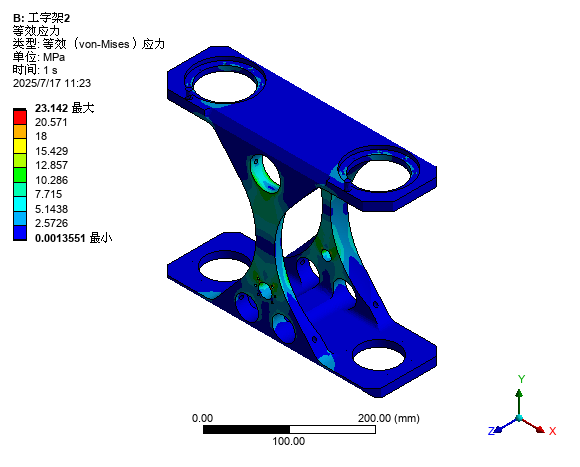
\includegraphics[width=\textwidth]{figures/chapter02/陀螺框架等效应力图.png}
    \caption{陀螺框架等效应力图}
    \label{陀螺框架等效应力图}
  \end{minipage}
  \hfill
  \begin{minipage}[t]{0.48\textwidth}
    \centering
    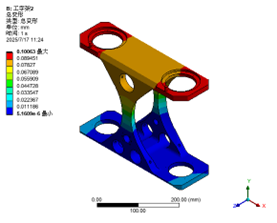
\includegraphics[width=\textwidth]{figures/chapter02/陀螺框架总变形图.png}
    \caption{陀螺框架总变形图}
    \label{陀螺框架总变形图}
  \end{minipage}
\end{figure}

（2）稳定模块的回形架

稳定模块的回形架主要承受力矩控制陀螺产生的控制扭矩以及以及陀螺装置和陀螺框架的重力。在模块安装支架空心轴支撑处施加CMG装置的重力载荷329.84N，并施加CMG装置产生的最大扭矩349.91Nm，结果如图\ref{模块安装支架等效应力图}和图\ref{模块安装支架总变形图}所示，最大等效应力仅为3.8654MPa，远小于材料屈服强度276MPa。最大变形仅为0.029mm，变形量极小，对整体结构性能影响可忽略不计。

\begin{figure}[!htbp]
  \centering
  \begin{minipage}[t]{0.48\textwidth}
    \centering
    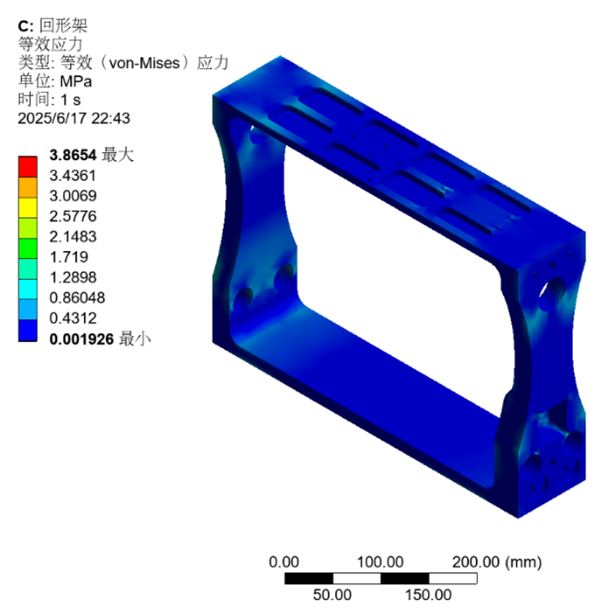
\includegraphics[width=\textwidth]{figures/chapter02/模块安装支架等效应力图.png}
    \caption{模块安装支架等效应力图}
    \label{模块安装支架等效应力图}
  \end{minipage}
  \hfill
  \begin{minipage}[t]{0.48\textwidth}
    \centering
    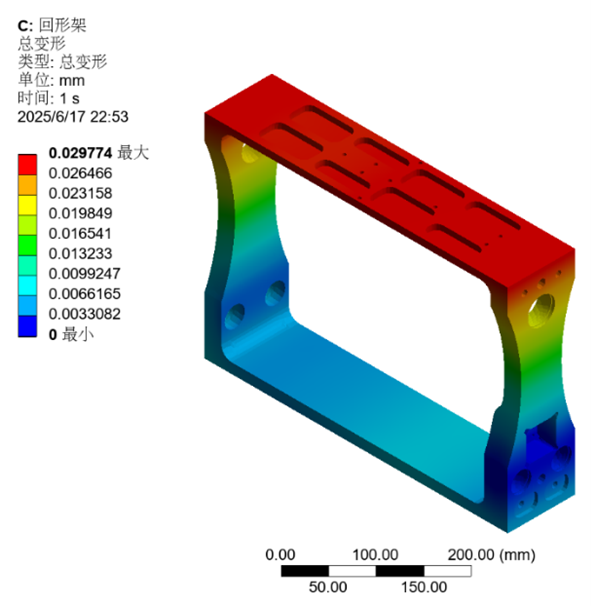
\includegraphics[width=\textwidth]{figures/chapter02/模块安装支架总变形图.png}
    \caption{模块安装支架总变形图}
    \label{模块安装支架总变形图}
  \end{minipage}
\end{figure}

（3）车体框架

对平衡车车体框架的主要结构进行装配有限元仿真。在连接架上施加981N（100kg）的载荷，在前、后侧板上施加稳定模块最大扭矩349.91Nm和稳定模块总重377.35N（38.46kg）的载荷且设置标准地球重力，并在车轮架的轮毂电机安装孔处设定固定支撑。由图\ref{车体框架等效应力图}和图\ref{车体框架总变形图}可以看出最大等效应力位于车轮架的转角处，数值为7.23MPa，远小于材料屈服强度276MPa；最大变形位于前后侧板顶端仅为0.063mm，对整体结构影响可忽略不计。

\begin{figure}[!htbp]
  \centering
  \begin{minipage}[t]{0.48\textwidth}
    \centering
    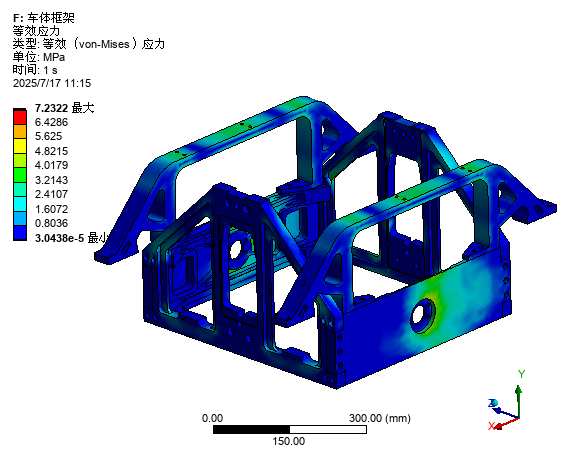
\includegraphics[width=\textwidth]{figures/chapter02/车体框架等效应力图.png}
    \caption{车体框架等效应力图}
    \label{车体框架等效应力图}
  \end{minipage}
  \hfill
  \begin{minipage}[t]{0.48\textwidth}
    \centering
    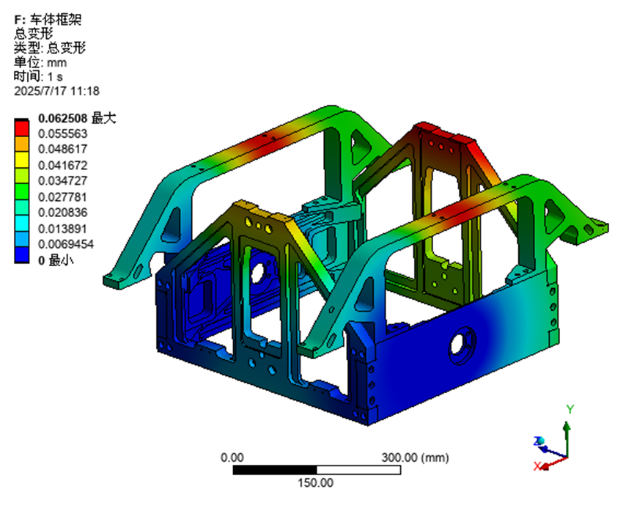
\includegraphics[width=\textwidth]{figures/chapter02/车体框架总变形图.png}
    \caption{车体框架总变形图}
    \label{车体框架总变形图}
  \end{minipage}
\end{figure}

\subsection{机械结构总成}

载人两轮平衡车的机械结构如图\ref{载人两轮平衡车三维模型}所示，连接了车体框架、稳定模块和驱动模块，具体包括了平衡车的轮毂电机、轮组、辅助轮、座椅、踏板及各种传感器。最终设计、装配好的两轮平衡车机械结构实物图如图\ref{平衡车机械结构装配实物图}所示。

\begin{figure}[!htbp]
  \centering
  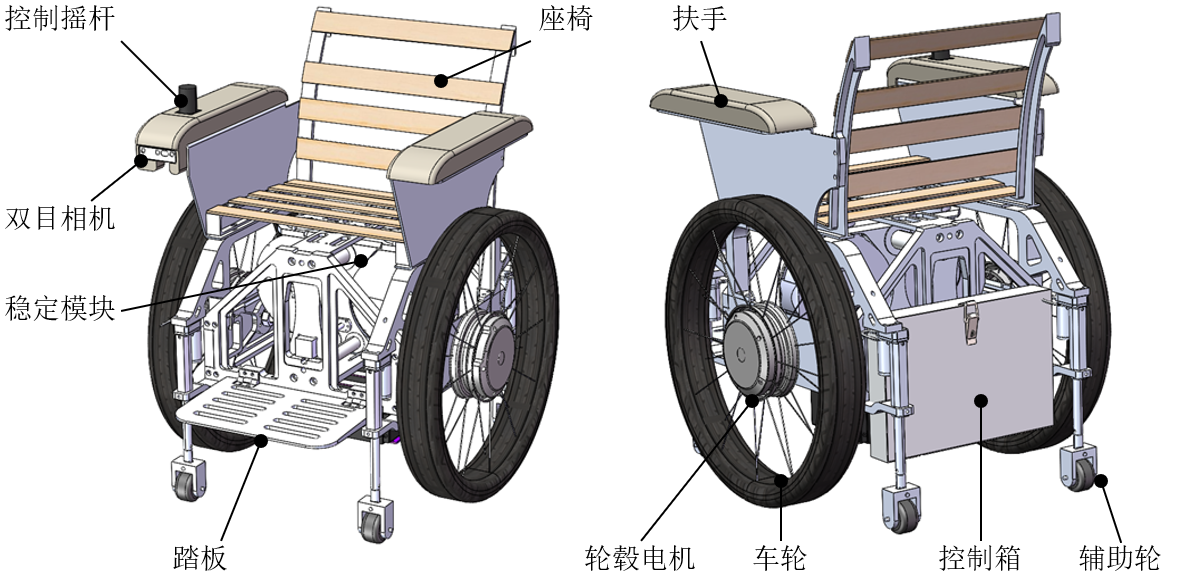
\includegraphics[width=0.85\textwidth]{figures/chapter02/两轮平衡车三维模型.png}
  \caption{载人两轮平衡车三维模型}
  \label{载人两轮平衡车三维模型}
\end{figure}

\begin{figure}[!htbp]
  \centering
  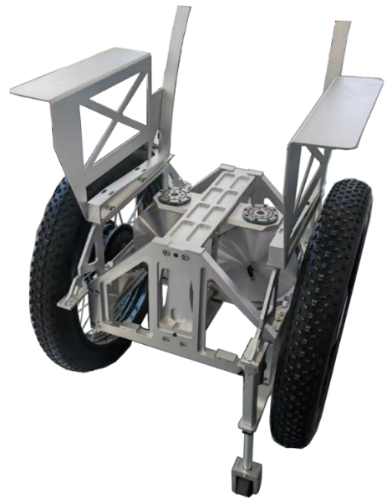
\includegraphics[width=0.48\textwidth]{figures/chapter02/机械装配实物图A.png}
  \hfill
  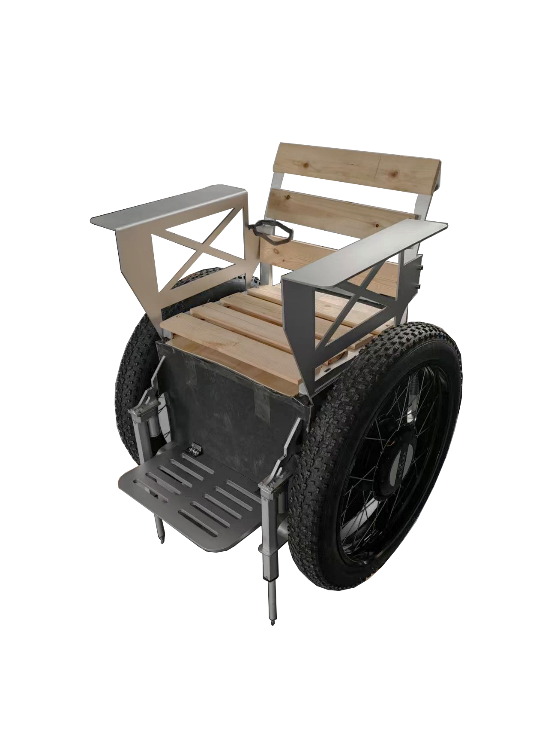
\includegraphics[width=0.48\textwidth]{figures/chapter02/机械装配实物图B.png}
  \caption{平衡车机械结构装配实物图}
  \label{平衡车机械结构装配实物图}
\end{figure}

\section{控制系统研究}

两轮平衡车的机械结构开发设计完后，需要对控制系统进行开发。首先根据控制需求完成控制方案的设计；然后进行硬件选型和硬件环境搭建；最后基于freeRTOS完成软件框架的搭建。

控制系统的方案如图\ref{控制系统方案}所示，主要由单片机、电机驱动器、传感器、控制器以及供电电路构成。控制系统一方面从上位机或控制器接收用户发出的运动指令，另一方面对姿态传感器、光电开关、编码器等传感器进行通讯采集，解算运动指令并进行平衡控制计算，然后通过驱动器生成各电机控制信号，实现精确运动控制。

\begin{figure}[!htbp]
  \centering
  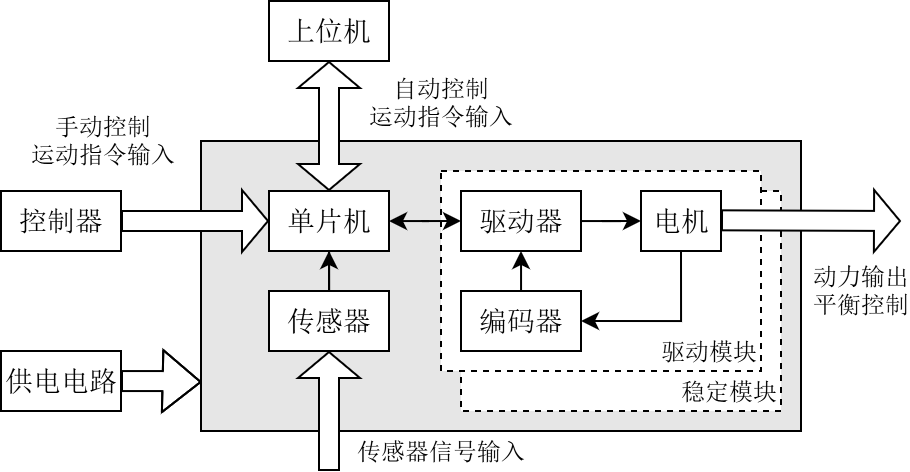
\includegraphics[width=0.85\textwidth]{figures/chapter02/控制系统方案.png}
  \caption{控制系统方案}
  \label{控制系统方案}
\end{figure}

\subsection{控制系统硬件设计}

控制系统的信号转换及电路连接如图\ref{控制系统信号电路连接}所示。基于控制任务的实时性与多通道控制需求，本设计选用STM32系列单片机作为控制器，通过网口、UART串口、CAN通讯、PWM输出以及GPIO等多种接口于其他元器件建立连接。

单片机通过以UDP协议为基础的网口通信方式与上位机建立高速连接，实现实时数据交换，在提升传输速率的同时，有效降低通信延迟，满足实时控制策略下对数据更新频率的严格要求。通过UART串口与控制器及姿态传感器进行通信，采集人工输入的控制指令及姿态信息。

为提升系统控制的总线统一性和抗干扰能力，除丝杠电机采用PWM方式进行控制外，其余电机驱动器均优先采用基于CAN总线的通信方式，以提高系统集成度并简化主控的通信负担。同时，通过GPIO接口接收丝杠电机光电开关的位置信号，实现对关键位置状态的快速响应与监测。

\begin{figure}[!htbp]
  \centering
  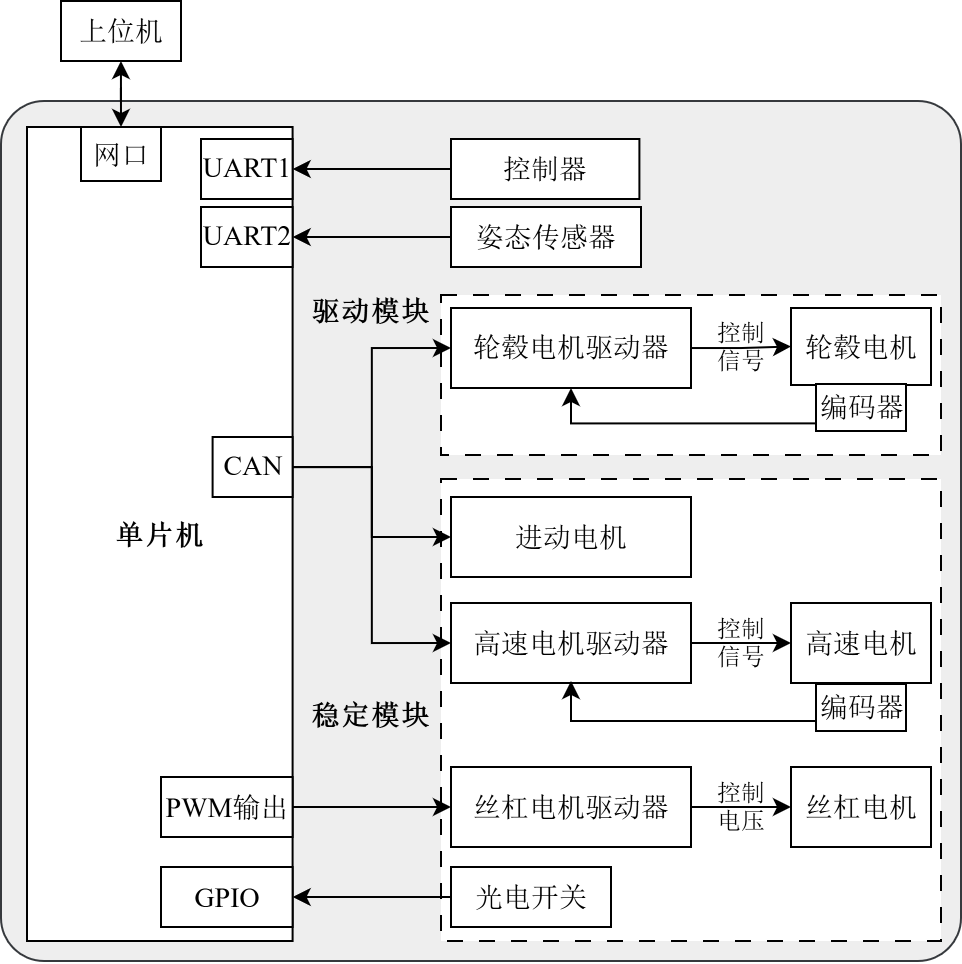
\includegraphics[width=0.70\textwidth]{figures/chapter02/控制系统信号电路连接.png}
  \caption{控制系统信号电路连接}
  \label{控制系统信号电路连接}
\end{figure}

控制系统的供电电路设计如图\ref{控制系统供电电路连接}所示。整车供电系统采用统一的48V直流电池电源作为主供电源，以简化能源分配结构并降低能量转换损耗。电源输出首先连接至一组继电保护模块，其中串联连接遥控继电器与手动电动开关，分别用于实现远程通断控制与现场物理切断，增强系统在调试、运行及紧急状态下的安全可控性。在主供电路径中，48V直流电压一方面直接分配至各电机驱动器为其提供高压高功率的驱动能源。另一方面经由降压转换模块变换后，输出24V直流电压供给单片机使用。单片机在正常运行时，通过其集成的稳压模块进一步输出5V直流电压，为系统中的姿态传感器、光电传感器和控制器提供稳定的低压电源。该分级供电设计有效隔离高低压系统，提升了电气系统的可靠性与抗干扰能力，亦为系统的维护与扩展提供了良好的电源接口基础。

\begin{figure}[!htbp]
  \centering
  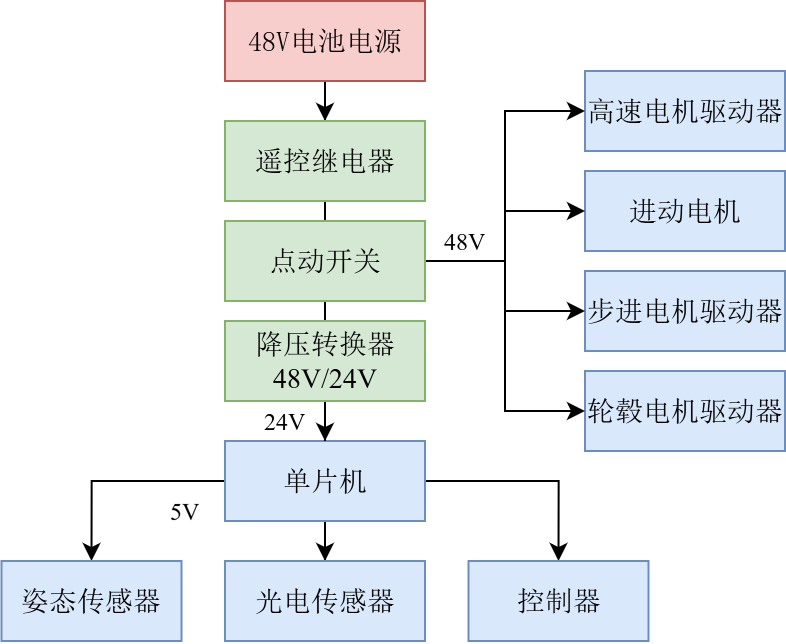
\includegraphics[width=0.85\textwidth]{figures/chapter02/控制系统电源电路连接.png}
  \caption{控制系统供电电路连接}
  \label{控制系统供电电路连接}
\end{figure}

\subsection{控制系统硬件环境搭建}

在控制系统主控芯片的选型中，重点从接口资源和控制能力两方面进行考量。接口方面，系统需通过网口采用UDP协议与上位机通信；同时需多个串口与手柄接收机、姿态传感器等模块通信，以及CAN接口以连接多个电机驱动器；此外，还需PWM通道控制丝杠电机，以及若干GPIO用于读取光电开关等传感器信号。控制方面，系统需要较强的实时处理能力和稳定的数据处理性能，以满足姿态计算和运动控制等任务。综合上述需求，最终选用挑选科鑫STM32F407ZGT6工控板作为控制器。该芯片集成网口、UART、双路CAN、丰富的PWM和GPIO资源，并搭载168MHz的Cortex-M4内核，配备1MB Flash和192KB SRAM，能够满足系统在通信、控制与实时性方面的各项要求。

\begin{figure}[!htbp]
  \centering
  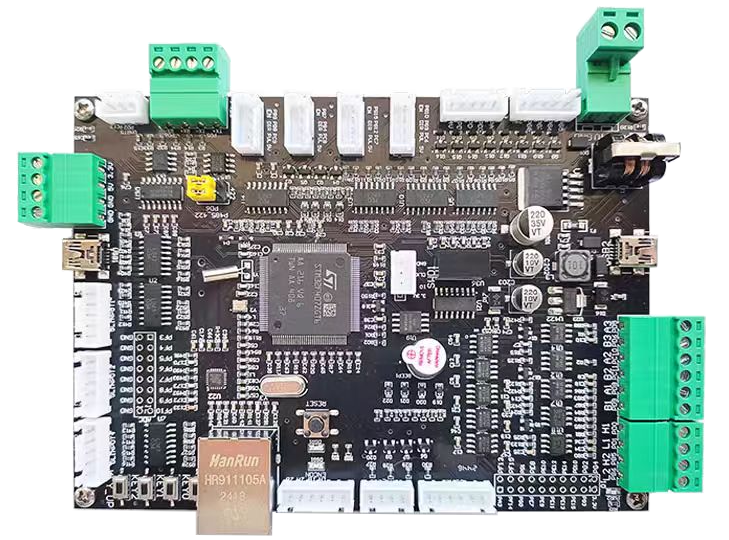
\includegraphics[width=0.85\textwidth]{figures/chapter02/STM32F407工业控制板.png}
  \caption{科鑫STM32F407ZGT6工控板}
  \label{科鑫STM32F407ZGT6工控板}
\end{figure}

姿态传感器需满足车辆对高频率、高精度姿态感知的需求。在本系统中，选用惯性测量单元（IMU）作为姿态传感器。IMU由三轴加速度计、三轴陀螺仪和三轴磁力计组成，通过对线加速度、角速度以及磁场等原始数据的采集，结合内置融合算法，实时计算出车辆的姿态角和角速度信息。综合考虑精度、响应速度、算法性能及系统兼容性，选用Wheeltec-H30惯性导航模块，其具备200Hz输出频率、0.1°角度分辨率，内置融合算法，可稳定输出姿态角与角速度，满足动态工况下的测量要求。

\begin{figure}[!htbp]
  \centering
  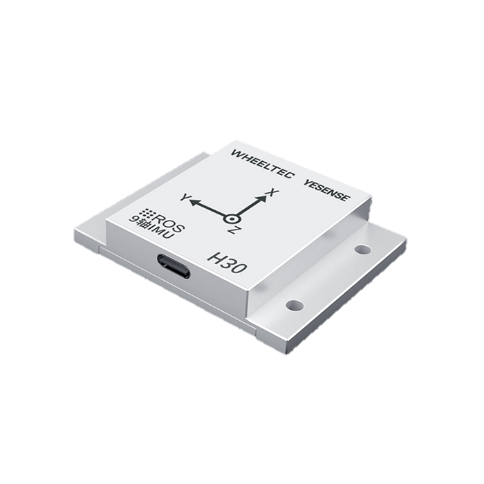
\includegraphics[width=0.70\textwidth]{figures/chapter02/维特智能H30惯导模块.png}
  \caption{Wheeltec-H30惯性导航模块}
  \label{Wheeltec-H30惯性导航模块}
\end{figure}

为满足开发阶段对整车控制与单电机调试的需求，系统需选用一款支持多通道输出、抗干扰强、通信稳定的控制手柄。综合性能与使用便利性，最终选用富斯FS-i6遥控器及其FS-iA10B接收模块，支持6通道以上模拟信号输出，具备拨码开关与自定义通道设置，可实现速度、角速度调节及电机独立控制，提升调试效率与系统灵活性。

\begin{figure}[!htbp]
  \centering
  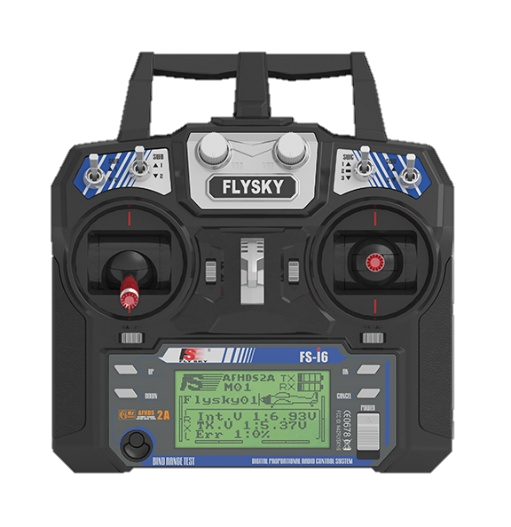
\includegraphics[width=0.68\textwidth]{figures/chapter02/FS-i6遥控器.png}
  \hfill
  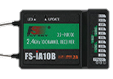
\includegraphics[width=0.22\textwidth]{figures/chapter02/FS-IA10B接收机模块.png}
  \caption{富斯FS-i6遥控器和FS-iA10B接收模块}
  \label{富斯FS-i6遥控器和FS-iA10B接收模块}
\end{figure}

为满足不同电机的驱动需求，系统依据性能参数选配匹配驱动器。轮毂电机采用中菱ZLAC8030L伺服驱动器，支持闭环控制和CAN通信，响应快速且抗干扰能力强；高速电机选用美固思MSSD-40LMA伺服驱动器，适配高速永磁同步电机，支持高频速度调节，也通过CAN总线通信；丝杠电机采用安川CA-4060M驱动器，采用PWM控制，支持多种模式及安全保护；进动电机为RobStride03一体式关节电机，内置驱动器，通过CAN总线直接与主控通信，简化布线并提升模块化。

搭建完成的控制系统主要部分电路如图\ref{控制系统连接实物图}所示，由于安装需要，惯性测量单元（IMU）和FS-iA10B接收模块在车体内部。

\begin{figure}[!htbp]
  \centering
  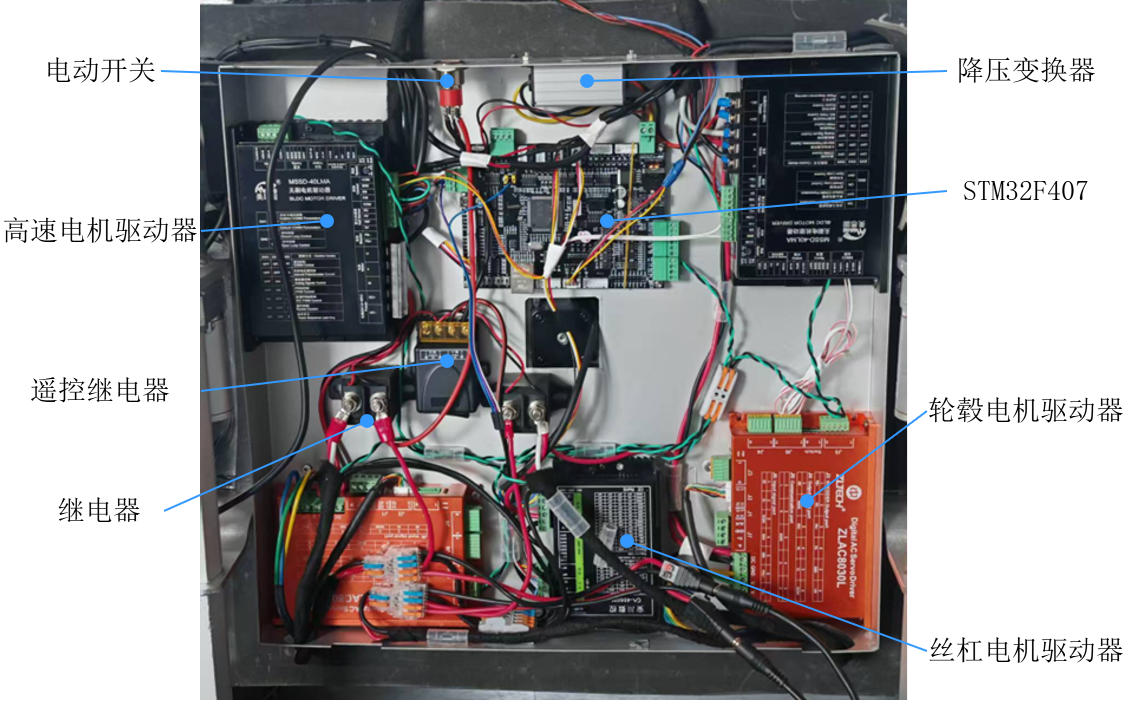
\includegraphics[width=0.85\textwidth]{figures/chapter02/控制系统实物连接图.png}
  \caption{控制系统连接实物图}
  \label{控制系统连接实物图}
\end{figure}

\subsection{控制系统软件总体方案设计}

（1）控制系统软件任务分析

在载人两轮平衡车的运行过程中，为确保系统的稳定性与乘员的安全性，系统必须实现多任务的实时并行处理。单片机作为底层控制核心，需要并发执行多项任务，主要包括设备通信、设备信息数据处理、运动控制计算、电机驱动控制以及状态反馈等。各项任务在实时性要求、驱动方式及执行周期上各不相同。其中，设备通信具有最高的实时性要求，通常采用中断方式进行，以实现与传感器、上位机等外部设备之间的快速响应与数据交换。设备信息数据处理、运动控制计算和电机驱动控制则属于中等实时性任务，通常以10ms的周期性方式执行，以确保对车体姿态变化的持续响应以及对电机的有效控制，从而维持系统平衡和运动性能。状态反馈任务则实时性要求较低，同样采用中断驱动方式，在系统资源允许的情况下进行调度即可。单片机需要执行的主要任务及其对应的实时性、驱动方式与运行周期如表\ref{控制系统软件任务分析}所示。

\begin{table}[!htbp]
  \centering
  \caption{控制系统软件任务分析}
  \label{控制系统软件任务分析}
  \vspace{0.5em}\wuhao
  \begin{tabularx}{\textwidth}{>{\centering\arraybackslash}X>{\centering\arraybackslash}X>{\centering\arraybackslash}X>{\centering\arraybackslash}X>{\centering\arraybackslash}X}
    \toprule
    编号 & 任务 & 实时性 & 驱动方式 & 运行周期 \\
    \midrule
    1 & 设备通信 & 高 & 中断 & 无 \\
    2 & 设备数据处理 & 中 & 周期 & 10ms \\
    3 & 运动控制计算 & 中 & 周期 & 10ms \\
    4 & 电机驱动控制 & 中 & 周期 & 10ms \\
    5 & 状态反馈 & 低 & 中断 & 无 \\
    \bottomrule
  \end{tabularx}
\end{table}

为了实现任务的高效调度与资源的合理分配，系统采用实时操作系统 FreeRTOS，结合STM32 HAL库，构建了轻量级、可扩展的多任务并行处理框架。由于系统中各类任务的实时性要求差异较大，尤其是姿态控制相关任务对确定性和响应速度要求高，基于中断或简单时间片轮转的调度机制难以满足其性能需求。

FreeRTOS提供了任务调度、优先级管理、定时器控制与资源同步等关键功能，能够有效协调多任务并发执行。系统将姿态数据读取、平衡控制计算、电机驱动、控制器信息接收、外部通信等功能划分为独立线程，并根据其实时性要求分配不同优先级，确保关键任务优先响应与执行，提升系统的实时性与可靠性。

为简化底层开发，提高代码可移植性与开发效率，系统引入了STM32 HAL库，通过统一的硬件抽象接口访问芯片资源。同时，采用STM32CubeIDE作为开发平台，借助其图形化配置、硬件配置代码自动生成与调试功能，规范并加速了开发流程。各模块间利FreeRTOS提供的消息队列、信号量等机制进行通信与协作，在保障关键控制流程快速响应的同时，也确保辅助任务的稳定运行，满足整车系统在复杂动态环境中的控制需求。

（2）软件系统总体框架及工作流程

控制系统的软件架构如图\ref{控制系统软件架构}所示采用分层设计，自上而下包括应用程序层、操作系统层、功能模块层和硬件驱动层。应用程序层实现系统的主要控制逻辑，任务包括设备数据处理、姿态估算、运动控制计算和电机控制命令生成。各功能以独立任务形式运行，满足周期性计算和实时控制的要求；操作系统层基于FreeRTOS，负责任务调度、定时器管理、中断处理和任务间通信（如信号量、消息队列等），用于协调各任务的运行顺序和资源使用；功能模块层根据各设备的API接口进行功能封装，为应用层提供统一的函数调用入口，上层可通过调用接口实现对IMU、电机、通信模块等的控制和数据获取；硬件驱动层运行在STM32平台上，使用HAL库访问GPIO、PWM、ADC、串口、CAN等外设资源，实现与传感器、电机和通信设备的底层交互。

\begin{figure}[!htbp]
  \centering
  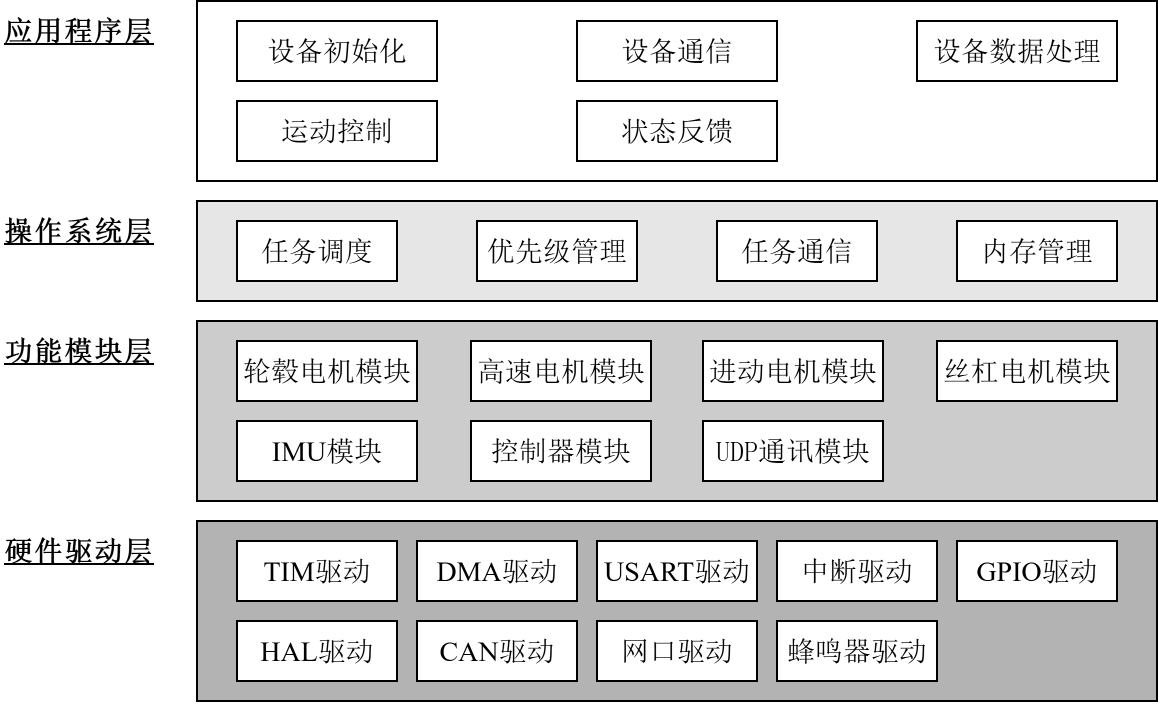
\includegraphics[width=0.85\textwidth]{figures/chapter02/控制系统软件架构.png}
  \caption{控制系统软件架构}
  \label{控制系统软件架构}
\end{figure}

控制系统的整体流程如图\ref{控制系统总体工作流程图}控制系统总体工作流程图所示。系统启动后，首先完成系统及各外设的初始化配置工作，包括传感器、执行器以及通信接口等模块的底层驱动加载与参数设置。初始化完成后，系统进入周期性调度的运行阶段，系统通过串口、CAN总线和UDP协议分别与IMU、各电机和上位机进行通信，获取实时数据。数据处理线程负责接收并处理来自IMU及各电机的反馈信息，将其转换为可用于控制的姿态和状态数据；运动控制线程则基于这些处理后的数据及上位机下发的运动指令，执行运动控制算法，生成相应的控制量并驱动各电机完成控制任务。

\begin{figure}[!htbp]
  \centering
  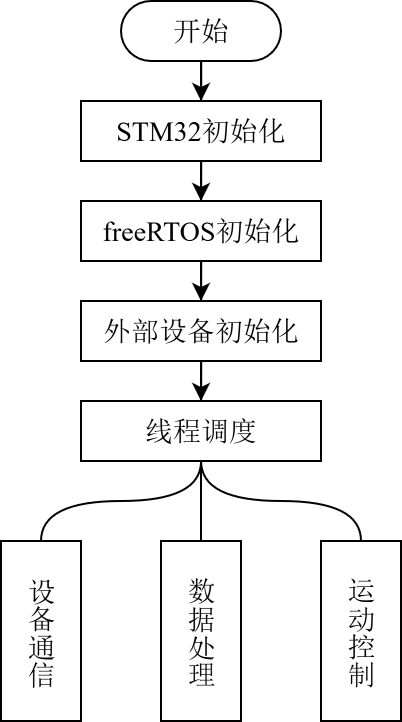
\includegraphics[width=0.45\textwidth]{figures/chapter02/控制系统总体流程.png}
  \caption{控制系统总体工作流程图}
  \label{控制系统总体工作流程图}
\end{figure}

\subsection{控制系统软件框架搭建}

（1）外部设备初始化流程

控制系统外部设备的初始化流程如图\ref{外部设备初始化流程}所示，主要包括外设通信初始化、电机初始化等内容。串口和CAN通信的中断需在初始化阶段手动开启，而以太网通信由驱动程序自动管理，无需人工干预。电机的初始化通过CAN总线完成，主要包括设置各电机的控制模式、目标位置以及执行回零操作，具体控制模式配置详见表\ref{电机控制模式设置}所示。此外，IMU（惯性测量单元）的滤波参数与输出配置由上位机完成设置；各电机的CAN通信地址同样由上位机下发设定。系统在初始化开始和结束时将通过蜂鸣器发出提示音，以提示操作人员当前状态。

\begin{table}[!htbp]
  \centering
  \caption{电机控制模式设置}
  \label{电机控制模式设置}
  \vspace{0.5em}\wuhao
  \begin{tabularx}{\textwidth}{>{\centering\arraybackslash}X>{\centering\arraybackslash}X}
    \toprule
    电机种类 & 控制模式 \\
    \midrule
    轮毂电机 & 力矩控制模式 \\
    进动电机 & 力矩控制模式 \\
    丝杠电机 & 脉冲控制模式 \\
    高速电机 & 位置控制模式 \\
    \bottomrule
  \end{tabularx}
\end{table}

\begin{figure}[!htbp]
  \centering
  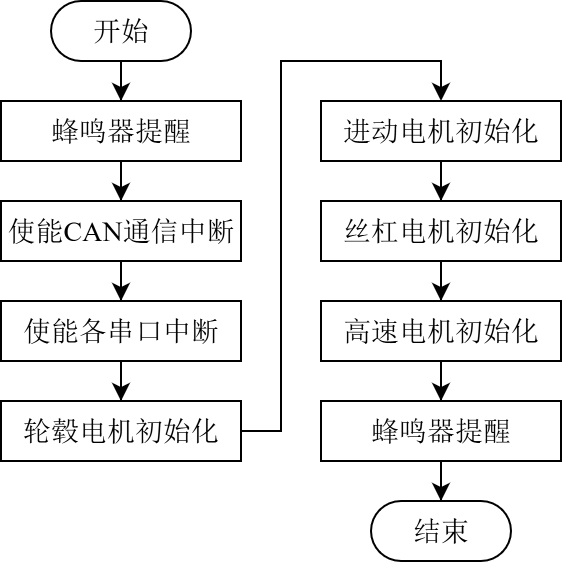
\includegraphics[width=0.70\textwidth]{figures/chapter02/外设初始化流程图.png}
  \caption{外部设备初始化流程}
  \label{外部设备初始化流程}
\end{figure}

（2）设备通信

在控制系统中，设备之间的通信通过串口、CAN和UDP三种方式实现：其中，两路串口分别用于与IMU及控制器的通信；CAN用于与各电机的通信；UDP 则用于与上位机进行数据交互。所有通信方式均基于中断机制实现数据接收与状态反馈。为了降低中断对系统线程调度的影响，中断服务程序中不直接处理数据内容，而仅负责接收数据及反馈当前通信状态。接收到的数据将被迅速转发至对应的消息队列，等待后续的数据处理线程按需读取并处理，从而提升系统整体的实时性与稳定性。

\begin{figure}[!htbp]
  \centering
  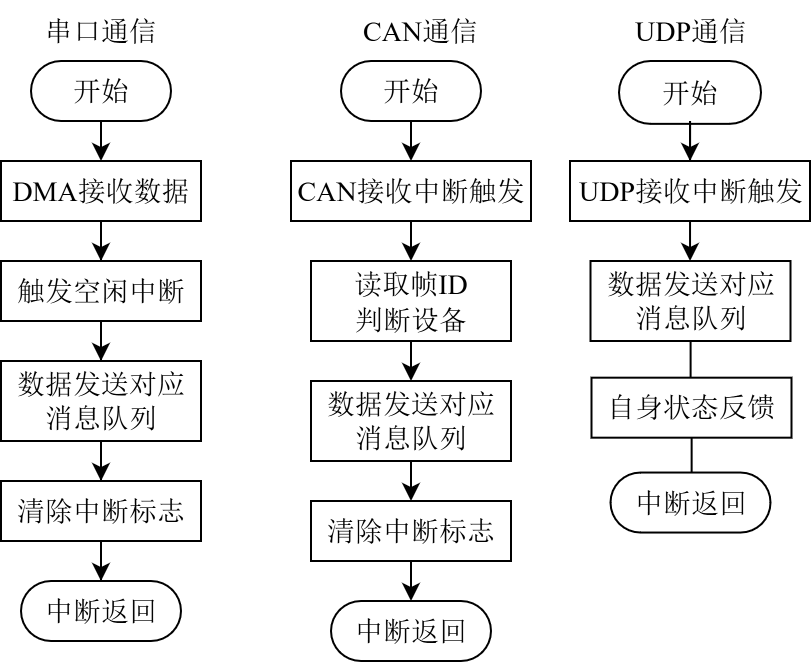
\includegraphics[width=0.85\textwidth]{figures/chapter02/设备通信流程图.png}
  \caption{控制系统设备通信流程图}
  \label{控制系统设备通信流程图}
\end{figure}

串口接收数据时，采用DMA（Direct Memory Access，直接存储器访问）方式将数据自动搬运至预设的内存缓冲区，无需CPU干预，从而显著减轻了处理负担并提升了搬运效率。当DMA正在接收数据过程中，若在设定的超时时间内未收到新的字节，即判定一帧数据接收完成，串口将触发空闲中断。中断服务程序在此时将DMA缓冲区中有效数据打包，并发送至对应的消息队列，供后台线程进一步解析处理。最后，清除中断标志，完成本次中断处理流程。

CAN通信主要用于与轮毂电机、高速电机和进动电机等部件之间的数据交互。系统启动后进入接收状态，当接收到来自电机的CAN数据帧时，将触发CAN接收中断。中断服务程序从接收缓冲区中读取数据帧内容，提取帧ID用以识别对应电机设备类型，并将数据发送至相应的数据处理消息队列，由后台线程异步完成后续解析与处理。最后，系统清除中断标志，完成本次中断处理流程。

UDP通信主要负责与自主导航系统之间的数据交互。当系统接收到来自导航系统的UDP数据报时，将立即触发相应的处理流程：首先将接收到的消息内容转发至指定的数据处理消息队列，供后台线程进行解析处理；随后，根据解析结果生成系统状态反馈报文并发送回上位机。反馈报文的具体结构如表\ref{状态反馈报文内容}所示。最后，完成当前UDP通信处理流程。

\begin{table}[!htbp]
  \centering
  \caption{状态反馈报文内容}
  \label{状态反馈报文内容}
  \vspace{0.5em}\wuhao
  \begin{tabularx}{\textwidth}{>{\centering\arraybackslash}X>{\centering\arraybackslash}X>{\centering\arraybackslash}X>{\centering\arraybackslash}X>{\centering\arraybackslash}X>{\centering\arraybackslash}X}
    \toprule
    Index & 说明 & 类型 & Index & 说明 & 类型 \\
    \midrule
    0 & 报文编号 & uint32\_t & 23 & 左侧轮毂电机当前转速 & float \\
    1–8 & 当前系统状态变量数组 & float[8] & 24 & 右侧轮毂电机当前转速 & float \\
    9 & 进动电机目标输出转矩 & float & 25 & 左侧轮毂电机电流 & float \\
    10 & 进动电机的目标转速 & float & 26 & 右侧轮毂电机电流 & float \\
    11 & 左侧进动电机角度 & float & 27 & 左侧高速电机转速 & float \\
    12 & 右侧进动电机角度 & float & 28 & 右侧高速电机转速 & float \\
    13 & 左侧进动电机速度 & float & 29 & 左侧高速电机电流 & float \\
    14 & 右侧进动电机速度 & float & 30 & 右侧高速电机电流 & float \\
    15 & 左侧进动电机输出转矩 & float & 31 & 左侧高速电机错误代码 & float \\
    16 & 右侧进动电机输出转矩 & float & 32 & 右侧高速电机错误代码 & float \\
    17 & 左侧进动电机温度 & float & 33 & 步进电机的目标位置 & float \\
    18 & 右侧进动电机温度 & float & 34 & 步进电机当前位置 & float \\
    19 & 左侧进动电机错误代码 & uint32\_t & 35 & 步进电机当前速度 & float \\
    20 & 右侧进动电机错误代码 & uint32\_t & 36 & 步进电机限位开关状态 & uint32\_t \\
    21 & 左侧轮毂电机目标转矩 & float & 37 & 数据校验码（16位CRC） & uint16\_t \\
    22 & 右侧轮毂电机目标转矩 & float & 38 & 测试字段 & uint16\_t \\
    \bottomrule
  \end{tabularx}
\end{table}

（3）设备数据处理

控制系统的设备数据处理流程如图\ref{控制系统设备数据处理流程}所示，主要功能是对各类外设传入的数据进行解析与管理。系统依次处理来自IMU、轮毂电机、高速电机、进动电机、控制器以及上位机的数据，按设定顺序从各数据队列获取数据并按照各设备的通信协议进行解析校验。

其中，IMU、轮毂电机、高速电机及进动电机的数据与车辆姿态平衡密切相关，对运行安全性影响较大。为保障系统的实时性与可靠性，若在解析过程中检测到上述关键设备的数据队列中无新数据，则系统将触发蜂鸣器报警，并记录对应的异常信息以供后续诊断。

\begin{figure}[!htbp]
  \centering
  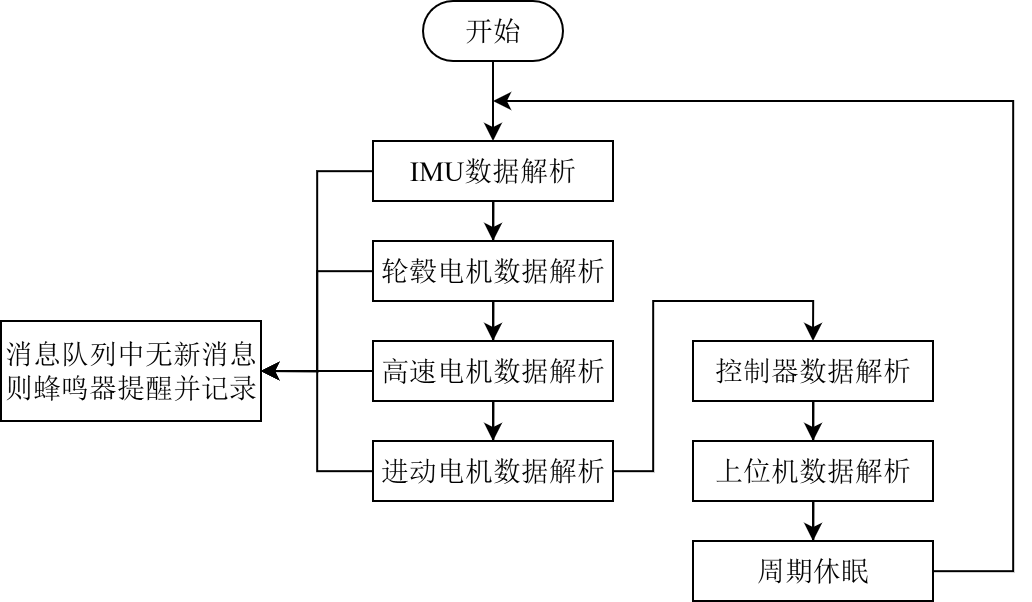
\includegraphics[width=0.85\textwidth]{figures/chapter02/设备数据处理流程图.png}
  \caption{控制系统设备数据处理流程}
  \label{控制系统设备数据处理流程}
\end{figure}

（4）运动控制

控制系统的运动控制流程如图\ref{控制系统运动控制流程图}所示。所设计的载人两人两轮平衡车搭载了力矩控制陀螺，在进行平衡控制前，需确保高速电机达到并维持在额定转速。因此，在运动控制线程启动后，系统首先通过遥控器判断是否进入运动控制状态；若需启动，则检测电机转速。若未达到额定转速，系统通过蜂鸣器提示异常，等待电机转速稳定。

当电机满足条件，系统进入由运动控制算法主导的控制阶段。该算法结合传感器反馈和运动指令，计算出控制策略并下发至电机控制模块，实现对电机的精确调节。控制完成后，系统进入周期性休眠，等待线程调度，形成稳定高效的实时闭环控制流程。控制系统的数据传输流程如图\ref{控制系统数据传输流程示意图}所示。

\begin{figure}[!htbp]
  \centering
  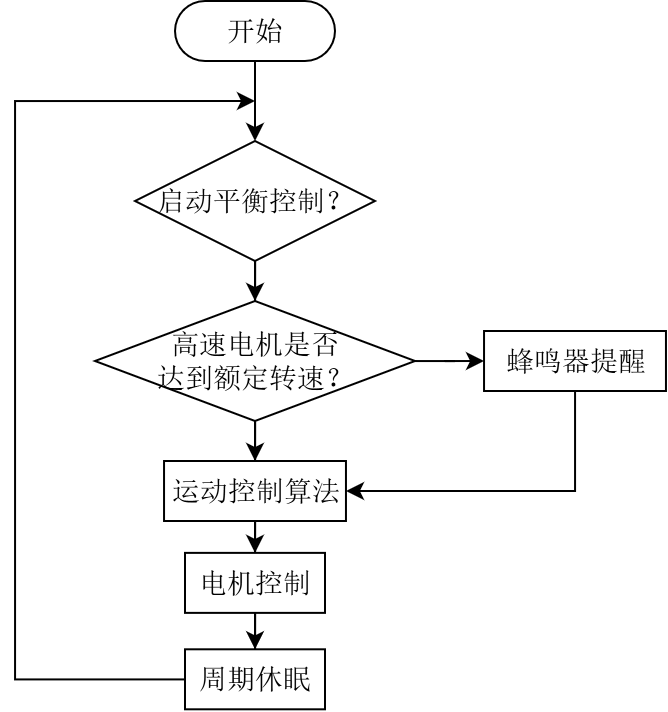
\includegraphics[width=0.68\textwidth]{figures/chapter02/运动控制流程图.png}
  \caption{控制系统运动控制流程图}
  \label{控制系统运动控制流程图}
\end{figure}

\begin{figure}[!htbp]
  \centering
  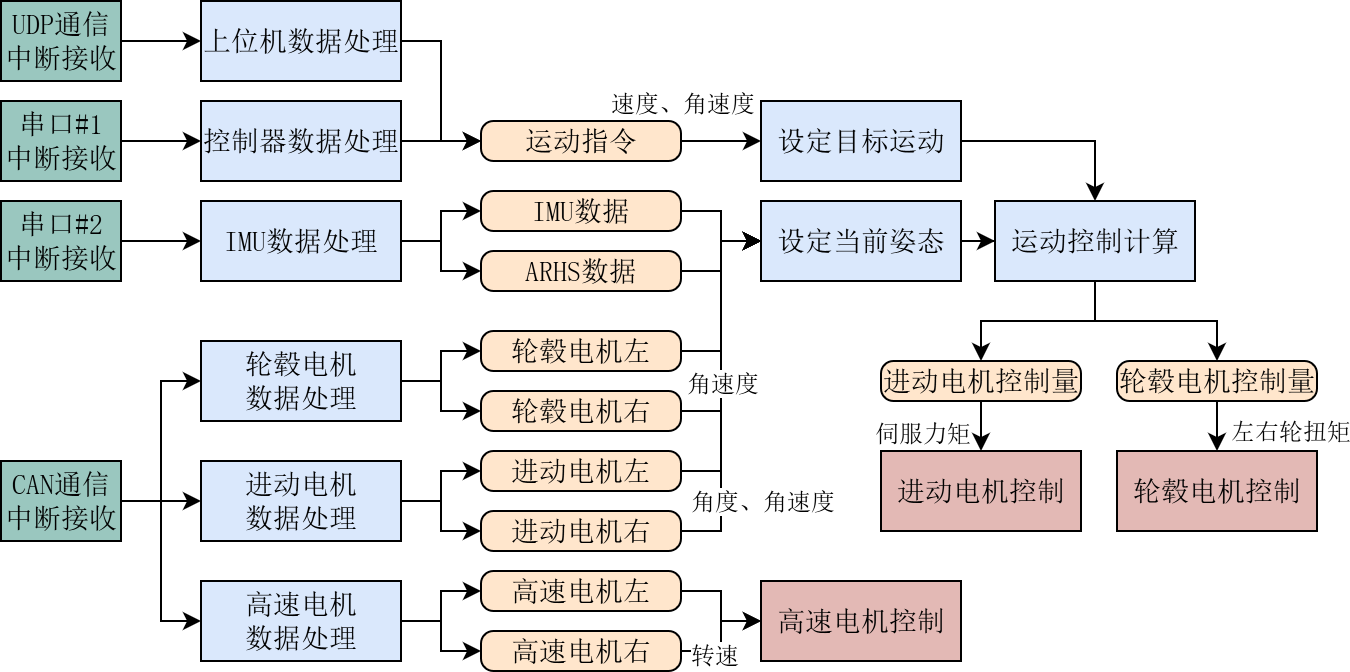
\includegraphics[width=0.85\textwidth]{figures/chapter02/数据传输流程图.png}
  \caption{控制系统数据传输流程示意图}
  \label{控制系统数据传输流程示意图}
\end{figure}

\subsection{本章小节}










